%
% File acl2018.tex
%
%% Based on the style files for ACL-2017, with some changes, which were, in turn,
%% Based on the style files for ACL-2015, with some improvements
%%  taken from the NAACL-2016 style
%% Based on the style files for ACL-2014, which were, in turn,
%% based on ACL-2013, ACL-2012, ACL-2011, ACL-2010, ACL-IJCNLP-2009,
%% EACL-2009, IJCNLP-2008...
%% Based on the style files for EACL 2006 by 
%%e.agirre@ehu.es or Sergi.Balari@uab.es
%% and that of ACL 08 by Joakim Nivre and Noah Smith

\documentclass[11pt,a4paper]{article}
\usepackage[hyperref]{acl2018}
\usepackage{times}
\usepackage{latexsym}
\newcommand\tab[1][1cm]{\hspace*{#1}}
\usepackage{url}
\usepackage{graphicx}

%\aclfinalcopy % Uncomment this line for the final submission
%\def\aclpaperid{***} %  Enter the acl Paper ID here

%\setlength\titlebox{5cm}
% You can expand the titlebox if you need extra space
% to show all the authors. Please do not make the titlebox
% smaller than 5cm (the original size); we will check this
% in the camera-ready version and ask you to change it back.

\newcommand\BibTeX{B{\sc ib}\TeX}

\title{Native Language Identification: Using Recurrent and Convolutional Neural Networks to Determine A Speaker's First Language}

\author{Lauren Becker, Daniel Brett, Isaiah Rawlinson, Clinton Tak}

\date{}

\begin{document}
\maketitle



\section{Introduction}
 Native Language Identification (NLI) is the process by which language production in a learned language (i.e. a secondary language) is used to identify an individual's native tongue. Typically, this classification task is framed where the set of native languages (L1 groups) are known a priori and classifiers are (usually) based on language-usage patterns that are endemic to specific L1 groups. For our experiment, our group utilized a corpus of essays from the CAES institute which are annotated for POS tags \footnote{See Data section for more specifics on essays.}. Using this data and the tensorflow library in python 3.6, our group used two types of neural nets as classifiers (CNN and RNN) and compared the accuracy of each. We then repeated this process using data from the Test of English as a Foreign Language (TOEFL) dataset\footnote{https://github.com/ClintonTak/NLP-Final-Projects/tree/master/Data/TOEFL} to see how our classifiers would perform with a larger corpus and a wider diversity of native languages.\\
 \tab The tasks of Native Language Identification has a number of applications, especially as it pertains to pedagogy, language transfer and forensic linguistics. By identifying L1-specific features, we can develop better teaching materials and perform author profiling.\footnote{Especially useful when attempting to determine who wrote an anonymous text, etc.} The latter of these two has proven so useful that it has attracted the attention of certain intelligence agencies which wish to harness NLI to learn more about threats and who are responsible for them. In essence, NLI has broad and potentially impactful applications.\\
 \tab Our groups has hypothesized that we can successfully build an NLI classification system using Annotated POS tags as vectors instead of the raw essays themselves. Typically, RNN's have been proven to be effective classifiers as it pertains to an NLI task (see literature reviews) so we believe that this classifier may provide better accuracy than a CNN.
 
 \section{Background: Literature Review}
 \subsection{Feature Analysis for Native Language Identification}
 \tab With the goal of demonstrating individuals of similar cultural backgrounds undergo overlapping language learning processes, Nisioi (2015)conducted multiple experiments with the EF Cambridge Open Language Database. Using 18 million tokens extracted from essays written by individuals from 29 separate countries, Nisioi extracted five distinct features for classification. These included POS n-grams, character n-grams, function words, shell nouns, and positional token frequency. Using an L2-Regularized L2-loss support vector classification machine, a log-entropy weighting scheme was used to construct feature vectors. 10-fold cross-validation experiments were then performed, yielding accuracy values like 99.89\% for character 4-grams, 97.42\% accuracy for positional tokens frequency, 96.22\% accuracy for function words and 93.65\% accuracy for shell nouns. POS tri-grams yielded a lower accuracy of 82.43\%. Regarding questions our group had, we were curious as to why the POS tri-grams yielded the lowest accuracy for the LB\_Ge dataset, but yielded the highest accuracy for the LB\_RuUk dataset. Is this a direct result of the structure of germanic languages versus English and Russian languages? Note that this article was helpful in helping us formulate our experiment because we thought that using an L-2 Regularized SVM as a classifier might be a good step going forward. While the classifiers we employ are all neural nets, we think it would be interesting ot see how the performance of an SVM would compare. 
 
 \subsection{Native Language Identification Shared Task}
 \tab In an effort to automatically identify the native languages (L1) of individuals based on their language production in a learned language, previous experiments have relied on classification tasks where the set of L1s is known a priori. Previous shared tasks have used data in the form of either essays or spoken responses, however Malmasi's 2017 experiment combines both of these inputs to build on the results from previous shared tasks. A large dataset called the TOEFL 11 was used to supply essays, speech transcripts, and audio features for dialect identification as well as a corpus consisting of both written essays and orthographic transcriptions of spoken responses obtained from test takers in the context of a standardized assessment. Prior to the experiment, the highest text-based accuracy was achieved by using features such as n-grams of words, parts-of-speech, and lemmas. The NLI Shared Task 2017 split their tasks into three parts consisting of text-only, audio-only, and fusion phases. A variety of classifier systems including ensembles and meta-classifiers were used and were the most effective in all tasks, with traditional classifiers such as SVMs with lexical syntactic features also incorporated throughout the experiment. Some of the takeaways from this experiment were that multiple classifier systems are very effective, lexical n-grams are the best single feature type, speech transcript features did not perform well, feature weighting schemes are important, and most importantly, combining written and spoken responses yields a higher prediction accuracy than other methods. While the formal academic context used to obtain the test data works within the scope of our project, it would be interesting to note how accuracy is affected by the context of the conversation. In the classroom foreign languages are often taught in a very formal manner, whereas conversational language can differ slightly in grammar and word usage. It would be interesting to see if less rehearsed conversational topics yield a higher accuracy for natural language identification assuming they uncover more grammatical errors than in formal conversation. It is also important to note that the experiment did not use raw audio data, making its inclusion in the speech and fusion tasks an interesting task in future research. This article provided helpful in formulating how we would test the accuracy of our classifier, specifically by using a priori one-hot vectors for each of the speaker's native languages, which we ultimately fed in to both our CNNs and RNNs.
 \subsection{Native Language Identification: SVMs vs. NNs}
 \tab Somsehkar et. all (2017) set out with the goal of determining whether an SVM or Neural Net is more effective at speakers with 11 different native languages. Using a publicly available dataset from ETS, the authors were able to reference 13,200 oral transcriptions (11,000 used for training, 1100 for dev, and 1100 for test sets) to use with their models. Advanced n-grams (unigrams and bigrams), spacy library (POS tagging), and i-vectors (high dimensional representations of speech) were used as features for both the Linear SVM and NN. The biggest gains for the SVM were reported when going from unigram to bigrams and adding i-vector data. Factoring in POS tags (surprisingly) did not significantly improve performance. Regarding the Neural Nets, the authors originally explored using RNNs, but eventually decided upon GRU cells as they achieved equal performance to LSTM cells, but had much lower training times. Using GLoVe vectors, the authors compiled accuracies for NN models. Overall, the models with the highest accuracies for SVMs and NNs (respectively) were the Stemmed words and i-vectors (0.802) and the GRU with GloVe and i-vecotrs (0.612). As we can see from these models, the linear SVM proved to be far more accurate, and the authors note that this was likely due to the vector embeddings. This article had an effect in how we outlined our experiment because it once again implied that SVM may be a more accurate classifier for this task. We hope to explore this classifier going forward.


\section{Data}
\subsection{Data Corpus}
\tab As mentioned in the introduction, our group utilized a corpus of essays from the CAES institute\footnote{URL: http://www.cervantes.es/default.htm}. These essays were annotated and converted into a set of language POS tags for all individuals in the database. All essays are written in Spanish. 
\subsection{Metadata and Associated Information}
\tab Data regarding the number of essays, languages and POS tags are outlined below:
\begin{center}
	\begin{tabular}{|c|c|}
		\hline
		Number of Respondents & 3878\\
		\hline
		Number of Essay Samples & 3878\\
		\hline
		Native Languages & French, Arabic,
		English, Russian\\
		& Portuguese, Chinese\\
		\hline
		Total Unique POS tags & 682172\\
		\hline
		Average Number of POS tags (per essay) & 175.9\\
		\hline
	\end{tabular}\\
	\textbf{Figure 1. Table With Basic Essay Information (CAES Institute)}
	
	\begin{center}
		\begin{tabular}{|c|c|}
			\hline
			Number of Respondents & 12100\\
			\hline
			Number of Essay Samples & 12100\\
			\hline
			Native Languages & German, Turkish, French, Arabic\\
			& Korean, Chinese, Hindi, Spanish \\
			& Italian, Japanese, Telugu\\
			\hline
			Total Unique POS tags & 26\\
			\hline
			Average Number of POS tags (per essay) & 341.9\\
			\hline
		\end{tabular}\\
		\textbf{Figure 2. Table With Basic Essay Information (TOEFL)}
	\end{center}
\end{center}
While the above figure contains basic information about the POS tags contained within each of the essays, our group also set out to learn more about the average number of POS tags for each native language. 
\begin{center}
	\begin{tabular}{|c|c|c|}
		\hline
		\textbf{Language} & \textbf{Total Responses} & \textbf{Average Number of POS Tags}\\
		\hline
		Arabic & 1342 & 148.3\\
		\hline
		Chinese & 373 & 169.3\\
		\hline
		English & 615 & 204.7\\
		\hline
		French & 371 & 189.5\\
		\hline
		Russian & 176 & 140.9\\
		\hline
		Portuguese & 1001 & 198.8\\
		\hline
	\end{tabular}
	\textbf{Figure 3. Metadata By Native Language (CAES Institute)}
\end{center}

\begin{center}
	\begin{tabular}{|c|c|c|}
		\hline
		\textbf{Language} & \textbf{Total Responses} & \textbf{Average Number of POS Tags}\\
		\hline
		German & 1100 & 369.1\\
		\hline
		Turkish & 1100 & 344.7\\
		\hline
		French & 1100 & 348.7\\
		\hline
		Arabic & 1100& 304.3\\
		\hline
		Korean & 1100& 331.3\\
		\hline
		Chinese & 1100 & 356.1\\
		\hline
		Hindi & 1100& 376.8\\
		\hline
		Spanish & 1100 & 354.0\\
		\hline
		Italian & 1100 & 316.9\\
		\hline
		Japanese & 1100 & 306.3\\
		\hline
		Telugu & 1100 & 353.6\\
		\hline
	\end{tabular}
	\textbf{Figure 4. Metadata By Native Language (TOEFL)}
\end{center}

\subsection{Preprocessing Methodology}
\tab Most of the pre-processing that our team needed to complete for this experiment required turning POS tags into vectors that our CNN/RNNs could accept. These steps are outlined\\
\\
1.) All distinct POS tags were scraped from the essays, put into a set, and then written to a file (done for both CAES and TOEFL).\\
2.) Each essays was then converted into a vector with each POS tag replaced by its index number from the first file.\\
3.) One hot vectors were then created for each of the languages. For each of the essays, depending on the native language a  one-hot vector was assigned to that essay (there were six different one hot vectors in CAES and 11 in TOEFL).\\
4.) Finally, to exclude outliers (i.e. incredibly short or long essays), essay vectors were limited by their size. For both the CAES and TOEFL vectors, this was anything bigger than 25 and smaller than 500. Graphs of the essay length distribution (before limiting length size) can be found below in \textbf{Figure 5} and \textbf{Figure 6.}
\begin{center}
	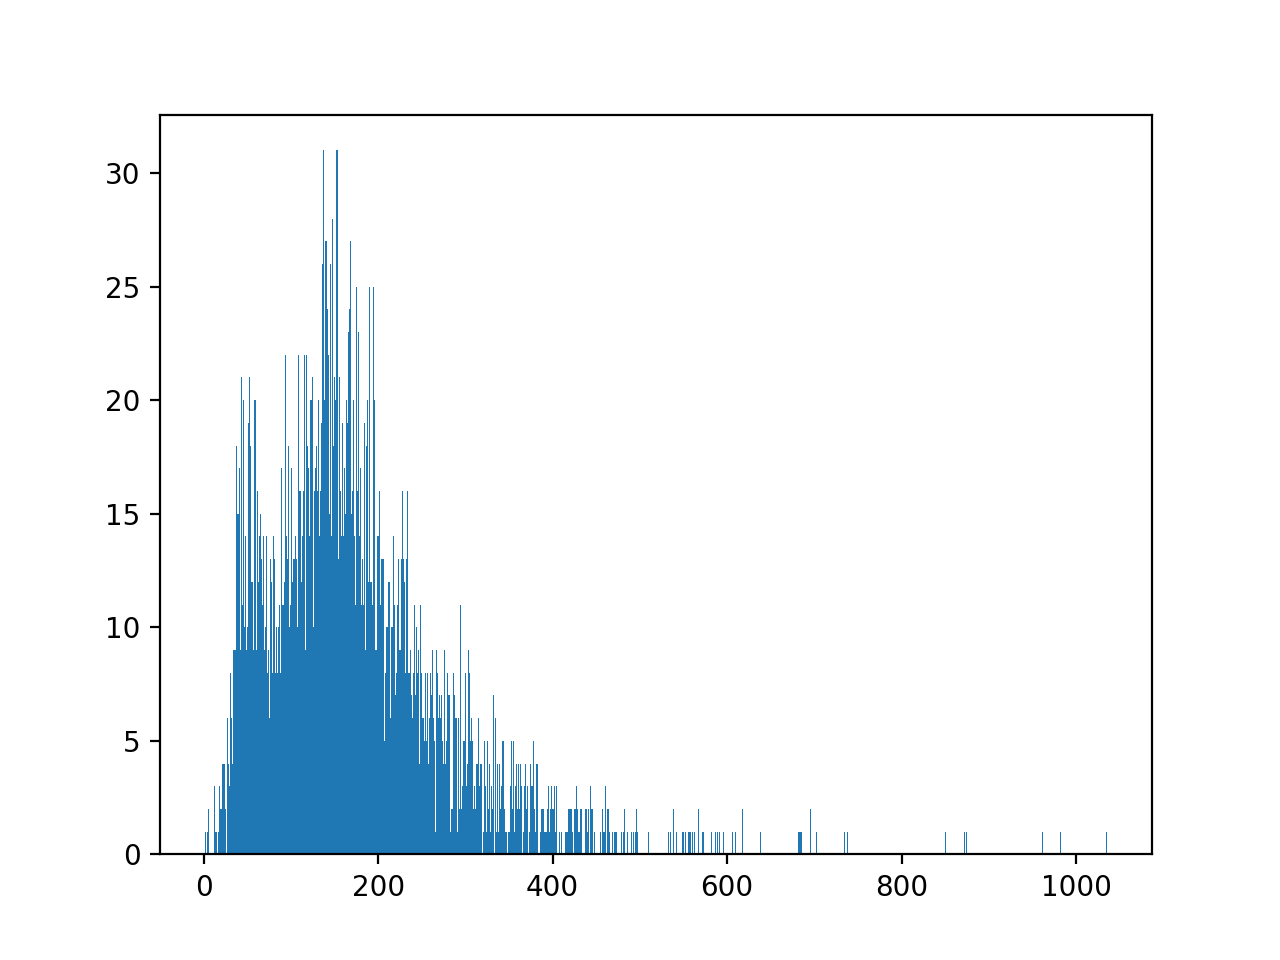
\includegraphics[scale=0.8]{lengthD}\\
	\textbf{Figure 5. Essay Length Distribution (CAES)}
	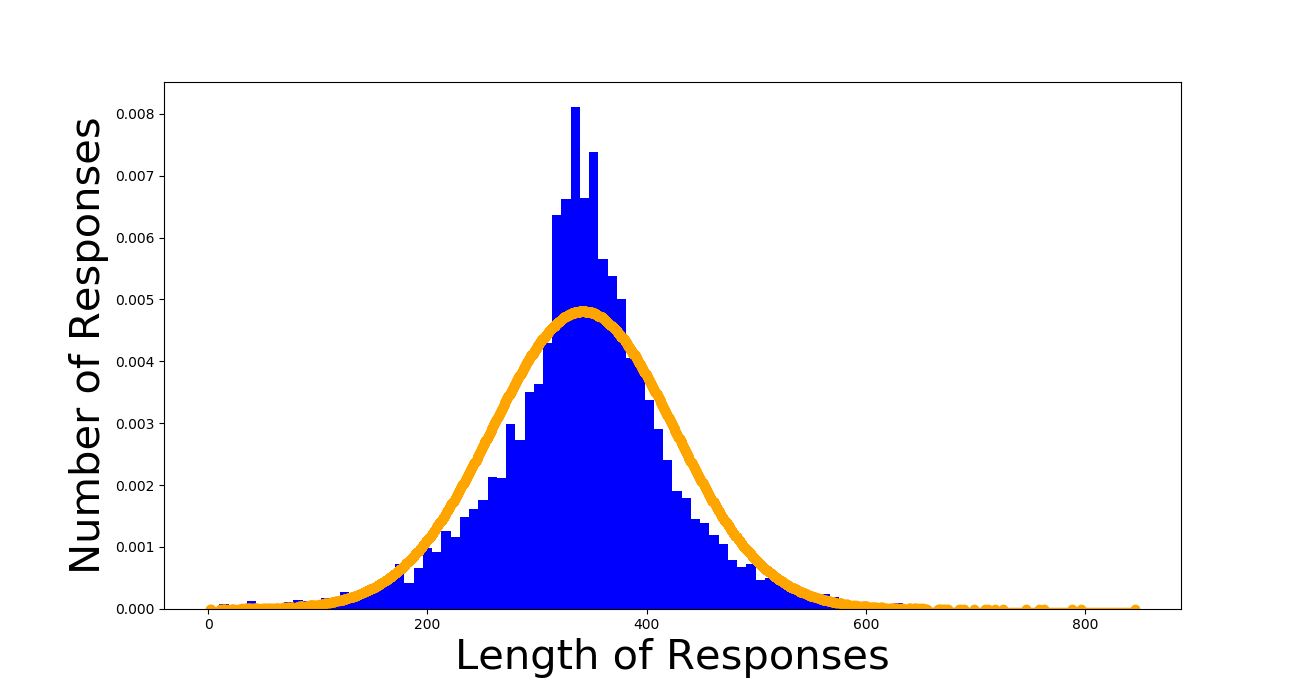
\includegraphics[scale=0.4]{Figure1}\\
	\textbf{Figure 6. Essay Length Distribution (TOEFL)}
\end{center}

\section{General Instructions}

Manuscripts must be in two-column format.  Exceptions to the
two-column format include the title, authors' names and complete
addresses, which must be centered at the top of the first page, and
any full-width figures or tables (see the guidelines in
Subsection~\ref{ssec:first}). \textbf{Type single-spaced.}  Start all
pages directly under the top margin. See the guidelines later
regarding formatting the first page.  The manuscript should be
printed single-sided and its length
should not exceed the maximum page limit described in Section~\ref{sec:length}.
Pages are numbered for  initial submission. However, \textbf{do not number the pages in the camera-ready version}.

By uncommenting {\verb|\aclfinalcopy|} at the top of this 
 document, it will compile to produce an example of the camera-ready formatting; by leaving it commented out, the document will be anonymized for initial submission.  When you first create your submission on softconf, please fill in your submitted paper ID where {\verb|***|} appears in the {\verb|\def\aclpaperid{***}|} definition at the top.

The review process is double-blind, so do not include any author information (names, addresses) when submitting a paper for review.  
However, you should maintain space for names and addresses so that they will fit in the final (accepted) version.  The ACL 2018 \LaTeX\ style will create a titlebox space of 6.35 cm for you when {\verb|\aclfinalcopy|} is commented out.  

\subsection{The Ruler}
The ACL 2018 style defines a printed ruler which should be present in the
version submitted for review.  The ruler is provided in order that
reviewers may comment on particular lines in the paper without
circumlocution.  If you are preparing a document without the provided
style files, please arrange for an equivalent ruler to
appear on the final output pages.  The presence or absence of the ruler
should not change the appearance of any other content on the page.  The
camera ready copy should not contain a ruler. (\LaTeX\ users may uncomment the {\verb|\aclfinalcopy|} command in the document preamble.)  

\textbf{Reviewers}: note that the ruler measurements do not align well with
lines in the paper -- this turns out to be very difficult to do well
when the paper contains many figures and equations, and, when done,
looks ugly. In most cases one would expect that the approximate
location will be adequate, although you can also use fractional
references ({\em e.g.}, the first paragraph on this page ends at mark $117.5$).

\subsection{Electronically-available resources}

ACL provides this description in \LaTeX2e{} ({\small\tt acl2018.tex}) and PDF
format ({\small\tt acl2018.pdf}), along with the \LaTeX2e{} style file used to
format it ({\small\tt acl2018.sty}) and an ACL bibliography style ({\small\tt acl\_natbib.bst})
and example bibliography ({\small\tt acl2018.bib}).
These files are all available at
\url{http://acl2018.org/downloads/acl18-latex.zip}.

A Microsoft Word template file ({\small\tt acl18-word.docx}) and example submission pdf ({\small\tt acl18-word.pdf})
is available at
\url{http://acl2018.org/downloads/acl18-word.zip}.
We strongly recommend the use of these style files, which have been
appropriately tailored for the ACL 2018 proceedings.

\subsection{Format of Electronic Manuscript}
\label{sect:pdf}

For the production of the electronic manuscript you must use Adobe's
Portable Document Format (PDF). PDF files are usually produced from
\LaTeX\ using the \textit{pdflatex} command. If your version of
\LaTeX\ produces Postscript files, you can convert these into PDF
using \textit{ps2pdf} or \textit{dvipdf}. On Windows, you can also use
Adobe Distiller to generate PDF.

Please make sure that your PDF file includes all the necessary fonts
(especially tree diagrams, symbols, and fonts with Asian
characters). When you print or create the PDF file, there is usually
an option in your printer setup to include none, all or just
non-standard fonts.  Please make sure that you select the option of
including ALL the fonts. \textbf{Before sending it, test your PDF by
  printing it from a computer different from the one where it was
  created.} Moreover, some word processors may generate very large PDF
files, where each page is rendered as an image. Such images may
reproduce poorly. In this case, try alternative ways to obtain the
PDF. One way on some systems is to install a driver for a postscript
printer, send your document to the printer specifying ``Output to a
file'', then convert the file to PDF.

It is of utmost importance to specify the \textbf{A4 format} (21 cm
x 29.7 cm) when formatting the paper. When working with
{\tt dvips}, for instance, one should specify {\tt -t a4}.
Or using the command \verb|\special{papersize=210mm,297mm}| in the latex
preamble (directly below the \verb|\usepackage| commands). Then using 
{\tt dvipdf} and/or {\tt pdflatex} which would make it easier for some.

Print-outs of the PDF file on A4 paper should be identical to the
hardcopy version. If you cannot meet the above requirements about the
production of your electronic submission, please contact the
publication chairs as soon as possible.

\subsection{Layout}
\label{ssec:layout}

Format manuscripts two columns to a page, in the manner these
instructions are formatted. The exact dimensions for a page on A4
paper are:

\begin{itemize}
\item Left and right margins: 2.5 cm
\item Top margin: 2.5 cm
\item Bottom margin: 2.5 cm
\item Column width: 7.7 cm
\item Column height: 24.7 cm
\item Gap between columns: 0.6 cm
\end{itemize}

\noindent Papers should not be submitted on any other paper size.
 If you cannot meet the above requirements about the production of 
 your electronic submission, please contact the publication chairs 
 above as soon as possible.

\subsection{Fonts}

For reasons of uniformity, Adobe's \textbf{Times Roman} font should be
used. In \LaTeX2e{} this is accomplished by putting

\begin{quote}
\begin{verbatim}
\usepackage{times}
\usepackage{latexsym}
\end{verbatim}
\end{quote}
in the preamble. If Times Roman is unavailable, use \textbf{Computer
  Modern Roman} (\LaTeX2e{}'s default).  Note that the latter is about
  10\% less dense than Adobe's Times Roman font.

\begin{table}[t!]
\begin{center}
\begin{tabular}{|l|rl|}
\hline \bf Type of Text & \bf Font Size & \bf Style \\ \hline
paper title & 15 pt & bold \\
author names & 12 pt & bold \\
author affiliation & 12 pt & \\
the word ``Abstract'' & 12 pt & bold \\
section titles & 12 pt & bold \\
subsection titles & 11 pt & bold \\
document text & 11 pt  &\\
captions & 11 pt & \\
abstract text & 11 pt & \\
bibliography & 10 pt & \\
footnotes & 9 pt & \\
\hline
\end{tabular}
\end{center}
\caption{\label{font-table} Font guide. }
\end{table}

\subsection{The First Page}
\label{ssec:first}

Center the title, author name(s), and affiliation(s) across both
columns (or, for the initial submission, \textbf{Anonymous ACL submission} for names and affiliations). Do not use footnotes for affiliations. 
Include the paper ID number assigned during the submission process in the header. 
Use the two-column format only when you begin the abstract.

\textbf{Title}: Place the title centered at the top of the first page, in
a 15-point bold font. (For a complete guide to font sizes and styles,
see Table~\ref{font-table}) Long titles should be typed on two lines
without a blank line intervening. Approximately, put the title at 2.5
cm from the top of the page, followed by a blank line, then the
author name(s), and the affiliation(s) on the following line. Do not
use only initials for given names (middle initials are allowed). Do
not format surnames in all capitals ({\em e.g.}, use ``Mitchell'' not
``MITCHELL'').  Do not format title and section headings in all
capitals as well except for proper names (such as ``BLEU'') that are
conventionally in all capitals.  The affiliation should contain the
author's complete address, and if possible, an electronic mail
address. Start the body of the first page 7.5 cm from the top of the
page.

The title, author names and addresses should be completely identical
to those entered to the electronic paper submission website in order
to maintain the consistency of author information among all
publications of the conference. If they are different, the publication
chairs may resolve the difference without consulting with you; so it
is in your own interest to double-check that the information is
consistent.

\textbf{Abstract}: Type the abstract at the beginning of the first
column. The width of the abstract text should be smaller than the
width of the columns for the text in the body of the paper by about
0.6 cm on each side. Center the word \textbf{Abstract} above the body of the abstract using the font size and style shown in Table~\ref{font-table}. The abstract should be a concise
summary of the general thesis and conclusions of the paper. It should
be no longer than 200 words. The font size of the abstract text should be as shown in Table~\ref{font-table}. 

\textbf{Text}: Begin typing the main body of the text immediately after
the abstract, observing the two-column format as shown in 
the present document. 
Do not include page numbers in the final version.

\textbf{Indent}: Indent when starting a new paragraph, about 0.4 cm.

%Use 11 points for text and subsection headings, 12 points for section headings and 15 points for the title. 


\begin{table}
\centering
\small
\begin{tabular}{cc}
\begin{tabular}{|l|l|}
\hline
\textbf{Command} & \textbf{Output}\\\hline
\verb|{\"a}| & {\"a} \\
\verb|{\^e}| & {\^e} \\
\verb|{\`i}| & {\`i} \\ 
\verb|{\.I}| & {\.I} \\ 
\verb|{\o}| & {\o} \\
\verb|{\'u}| & {\'u}  \\ 
\verb|{\aa}| & {\aa}  \\\hline
\end{tabular} & 
\begin{tabular}{|l|l|}
\hline
\textbf{Command} & \textbf{ Output}\\\hline
\verb|{\c c}| & {\c c} \\ 
\verb|{\u g}| & {\u g} \\ 
\verb|{\l}| & {\l} \\ 
\verb|{\~n}| & {\~n} \\ 
\verb|{\H o}| & {\H o} \\ 
\verb|{\v r}| & {\v r} \\ 
\verb|{\ss}| & {\ss} \\\hline
\end{tabular}
\end{tabular}
\caption{Example commands for accented characters, to be used in, {\em e.g.}, \BibTeX\ names.}\label{tab:accents}
\end{table}

\subsection{Sections}

\textbf{Headings}: Type and label section and subsection headings in the
style shown on the present document.  Use numbered sections (Arabic
numerals) in order to facilitate cross references. Number subsections
with the section number and the subsection number separated by a dot, in Arabic numerals. 
Do not number subsubsections ({\em i.e.}, use \verb|\subsubsection*| instead of \verb|\subsubsection|).

\begin{table*}
\centering
\begin{tabular}{lll}
  output & natbib & previous ACL style files\\
  \hline
  \citep{Gusfield:97} & \verb|\citep| & \verb|\cite| \\
  \citet{Gusfield:97} & \verb|\citet| & \verb|\newcite| \\
  \citeyearpar{Gusfield:97} & \verb|\citeyearpar| & \verb|\shortcite| \\
\end{tabular}
\caption{Citation commands supported by the style file.
  The citation style is based on the natbib package and
  supports all natbib citation commands.
  It also supports commands defined in previous ACL style files
  for compatibility.
  }
\end{table*}

\textbf{Citations}: Citations within the text appear in parentheses
as~\cite{Gusfield:97} or, if the author's name appears in the text
itself, as Gusfield~\shortcite{Gusfield:97}.
Using the provided \LaTeX\ style, the former is accomplished using
{\verb|\cite|} and the latter with {\verb|\shortcite|} or {\verb|\newcite|}.
Collapse multiple citations as in~\cite{Gusfield:97,Aho:72}; this is accomplished with the provided style using commas within the {\verb|\cite|} command, {\em e.g.}, {\verb|\cite{Gusfield:97,Aho:72}|}.  
Append lowercase letters to the year in cases of ambiguities.  
 Treat double authors as
in~\cite{Aho:72}, but write as in~\cite{Chandra:81} when more than two
authors are involved. 
%Collapse multiple citations as
%in~\cite{Gusfield:97,Aho:72}. 

Also refrain from using full citations
as sentence constituents.
%\penalty -5000
We suggest that instead of
\begin{quote}
  ``\cite{Gusfield:97} showed that ...''
\end{quote}
you use
\begin{quote}
``Gusfield \shortcite{Gusfield:97}   showed that ...''
\end{quote}

If you are using the provided \LaTeX{} and Bib\TeX{} style files, you
can use the command \verb|\citet| (cite in text)
to get ``author (year)'' citations.

You can use the command \verb|\citealp| (alternative cite without 
parentheses) to get ``author year'' citations (which is useful for 
using citations within parentheses, as in \citealp{Gusfield:97}).

If the Bib\TeX{} file contains DOI fields, the paper
title in the references section will appear as a hyperlink
to the DOI, using the hyperref \LaTeX{} package.
To disable the hyperref package, load the style file
with the \verb|nohyperref| option:
\verb|\usepackage[nohyperref]{acl2018}|.

\textbf{Compilation Issues}: Some of you might encounter the following error during compilation: 

``{\em \verb|\pdfendlink| ended up in different nesting level than \verb|\pdfstartlink|.}''

This happens when \verb|pdflatex| is used and a citation splits across a page boundary. To fix this, disable the \verb|hyperref| package (see above), recompile and see the problematic citation.
Next rewrite that sentence containing the citation. (See, {\em e.g.}, {\small\tt http://tug.org/errors.html})

\textbf{Digital Object Identifiers}:  As part of our work to make ACL
materials more widely used and cited outside of our discipline, ACL
has registered as a CrossRef member, as a registrant of Digital Object
Identifiers (DOIs), the standard for registering permanent URNs for
referencing scholarly materials. We are requiring all
camera-ready references to contain the appropriate DOIs (or as a
second resort, the hyperlinked ACL Anthology Identifier) to all cited
works.  Thus, please ensure that you use Bib\TeX\ records that contain
DOI or URLs for any of the ACL materials that you reference.
Appropriate records should be found for most materials in the current
ACL Anthology at \url{http://aclanthology.info/}.

As examples, we cite \cite{P16-1001} to show you how papers with a DOI
will appear in the bibliography.  We cite \cite{C14-1001} to show how
papers without a DOI but with an ACL Anthology Identifier will appear
in the bibliography.  

As reviewing will be double-blind, the submitted version of the papers
should not include the authors' names and affiliations. Furthermore,
self-references that reveal the author's identity, {\em e.g.},
\begin{quote}
``We previously showed \cite{Gusfield:97} ...''  
\end{quote}
should be avoided. Instead, use citations such as 
\begin{quote}
``\citeauthor{Gusfield:97} \shortcite{Gusfield:97}
previously showed ... ''
\end{quote}

\textbf{Please do not use anonymous citations} and do not include
acknowledgments when submitting your papers. Papers that do not
conform to these requirements may be rejected without review.

\textbf{References}: Gather the full set of references together under
the heading \textbf{References}. 
Arrange the references alphabetically
by first author, rather than by order of occurrence in the text.
Provide as complete a citation as possible, using a consistent format,
such as the one for {\em Computational Linguistics\/} or the one in the 
{\em Publication Manual of the American 
Psychological Association\/}~\cite{APA:83}.  Use of full names for
authors rather than initials is preferred.
A list of abbreviations for common computer science journals can be found in the ACM {\em Computing Reviews\/}~\cite{ACM:83}.

The \LaTeX{} and Bib\TeX{} style files provided roughly fit the
American Psychological Association format, allowing regular citations, 
short citations and multiple citations as described above.

\subsection{Footnotes}

\textbf{Footnotes}: Put footnotes at the bottom of the page and use the footnote font size shown in Table~\ref{font-table}. They may be numbered or referred to by asterisks or other
symbols.\footnote{This is how a footnote should appear.} Footnotes
should be separated from the text by a line.\footnote{Note the line
separating the footnotes from the text.}

\subsection{Figures and Tables}

%\textbf{Placement}: Place figures and tables in the
%paper near where they are first discussed if
%possible.  
%Wide figures and tables may run across both columns and should be placed at the top of a page.

\textbf{Placement}: Place figures and tables in the paper near where they are first discussed, as close as possible to the top of their respective column.

%Color illustrations are discouraged, unless you have verified that  
%they will be understandable when printed in black ink.

\textbf{Captions}: Provide a caption for every illustration; number each one
sequentially in the form:  ``Figure 1: Caption of the Figure.'' ``Table 1:
Caption of the Table.''  Type the captions of the figures and 
tables below the body, using the caption font size shown in Table~\ref{font-table}.

\subsection{Equation}
\label{ssec:eqn}

An example equation is shown below:
\begin{equation}
A=\pi r^2
\end{equation}

The numbering (if any) and alignment of the equations will be done automatically (using \verb|align| or \verb|equation|).

\subsection{Accessibility}
\label{ssec:accessibility}

In an effort to accommodate the color-blind (as well as those printing
to paper), grayscale readability for all accepted papers will be
encouraged.  Color is not forbidden, but authors should ensure that
tables and figures do not rely solely on color to convey critical
distinctions.
A simple criterion: All curves and points in your figures should be clearly distinguishable without color.
%Here we give a simple criterion on your colored figures, if your paper has to be printed in black and white, then you must assure that every curves or points in your figures can be still clearly distinguished.

% Min: no longer used as of ACL 2017, following ACL exec's decision to
% remove this extra workflow that was not executed much.
% BEGIN: remove
%% \section{XML conversion and supported \LaTeX\ packages}

%% Following ACL 2014 we will also we will attempt to automatically convert 
%% your \LaTeX\ source files to publish papers in machine-readable 
%% XML with semantic markup in the ACL Anthology, in addition to the 
%% traditional PDF format.  This will allow us to create, over the next 
%% few years, a growing corpus of scientific text for our own future research, 
%% and picks up on recent initiatives on converting ACL papers from earlier 
%% years to XML. 

%% We encourage you to submit a ZIP file of your \LaTeX\ sources along
%% with the camera-ready version of your paper. We will then convert them
%% to XML automatically, using the LaTeXML tool
%% (\url{http://dlmf.nist.gov/LaTeXML}). LaTeXML has \emph{bindings} for
%% a number of \LaTeX\ packages, including the ACL 2017 stylefile. These
%% bindings allow LaTeXML to render the commands from these packages
%% correctly in XML. For best results, we encourage you to use the
%% packages that are officially supported by LaTeXML, listed at
%% \url{http://dlmf.nist.gov/LaTeXML/manual/included.bindings}
% END: remove

\section{Translation of non-English Terms}

It is also advised to supplement non-English characters and terms
with appropriate transliterations and/or translations
since not all readers understand all such characters and terms.
Inline transliteration or translation can be represented in
the order of: original-form transliteration ``translation''.

\section{Length of Submission}
\label{sec:length}

The ACL 2018 main conference accepts submissions of long papers and
short papers.
 Long papers may consist of up to eight (8) pages of
content plus unlimited pages for references. Upon acceptance, final
versions of long papers will be given one additional page -- up to nine (9)
pages of content plus unlimited pages for references -- so that reviewers' comments
can be taken into account. Short papers may consist of up to four (4)
pages of content, plus unlimited pages for references. Upon
acceptance, short papers will be given five (5) pages in the
proceedings and unlimited pages for references. 

For both long and short papers, all illustrations and tables that are part
of the main text must be accommodated within these page limits, observing
the formatting instructions given in the present document. 
Papers that do not conform to the specified length and 
formatting requirements are subject to be rejected without
review.

Workshop chairs may have different rules for allowed length and
whether supplementary material is welcome. As always, the respective
call for papers is the authoritative source.

\section{Supplementary Material}
\label{sec:supplemental}
ACL 2018 also encourages the submission of supplementary material
to report preprocessing decisions, model parameters, and other details
necessary for the replication of the experiments reported in the 
paper. Seemingly small preprocessing decisions can sometimes make
a large difference in performance, so it is crucial to record such
decisions to precisely characterize state-of-the-art methods.

Nonetheless, supplementary material should be supplementary (rather
than central) to the paper. \textbf{Submissions that misuse the supplementary 
material may be rejected without review.}
Essentially, supplementary material may include explanations or details
of proofs or derivations that do not fit into the paper, lists of
features or feature templates, sample inputs and outputs for a system,
pseudo-code or source code, and data. 

The paper should not rely on the supplementary material: while the paper
may refer to and cite the supplementary material and the supplementary material will be available to the
reviewers, they will not be asked to review the
supplementary material.

The supplementary material does not form part of the paper, does not count towards the page limit, and should not be included in an ``Appendix'' section following the references in this template. The ``container'' for supplementary materials is a separate document, and such materials should be submitted separately from the paper using the appropriate fields on the review form and the camera-ready upload form. 

\section*{Acknowledgments}

The acknowledgments should go immediately before the references.  Do not number the acknowledgments section ({\em i.e.}, use \verb|\section*| instead of \verb|\section|). Do not include this section when submitting your paper for review.

% include your own bib file like this:
%\bibliographystyle{acl}
%\bibliography{acl2018}
\bibliography{acl2018}
\bibliographystyle{acl_natbib}

\end{document}
